\appendix
\chapter{Mathematical Toolkit for Data Science}
\label{app:math-toolkit}

This appendix collects the mathematical ideas repeatedly used throughout the course. It is intended as a visual reference rather than a substitute for a full probability, statistics, or linear-algebra course. The goal is to connect formulas to the data-science operations they support.

\section{Notation: observations, features, and matrices}
For a dataset with $n$ observations and $p$ numeric features, it is convenient to write the feature matrix as
\[
X=\begin{bmatrix}
 x_{11} & x_{12} & \cdots & x_{1p}\\
 x_{21} & x_{22} & \cdots & x_{2p}\\
 \vdots & \vdots & \ddots & \vdots\\
 x_{n1} & x_{n2} & \cdots & x_{np}
\end{bmatrix}.
\]
One row is an observation vector; one column is a feature vector. A supervised target is often written $\mathbf{y}=(y_1,\ldots,y_n)^T$.

\begin{utpfig}[Rows and columns become vectors]{Matrix notation is compact, but it still represents the same rows and columns used in a data frame.}{fig:math-matrix}
\begin{tikzpicture}[x=\linewidth,y=1cm,
  entry/.style={draw=UTPBlue!60,fill=UTPPaleBlue,rounded corners=1mm,
    line width=0.5pt,text width=0.065\linewidth,minimum height=0.55cm,
    inner xsep=1mm,inner ysep=1mm,align=center,
    font=\scriptsize\color{UTPNavy}},
  labeltext/.style={font=\scriptsize\color{UTPNavy},align=left,
    text width=0.28\linewidth,anchor=west,inner sep=0pt}]
\foreach \r in {1,...,5}{
  \foreach \c in {1,...,6}{
    \node[entry] (x-\r-\c) at (0.10*\c,-0.72*\r) {$x_{\r\c}$};
  }
}
\draw[draw=UTPOrange!85!black,line width=1pt,rounded corners=1.5mm]
  ([xshift=-1mm,yshift=1mm]x-1-1.north west) rectangle
  ([xshift=1mm,yshift=-1mm]x-1-6.south east);
\draw[draw=UTPTeal!85!black,line width=1pt,rounded corners=1.5mm]
  ([xshift=-1mm,yshift=1mm]x-1-3.north west) rectangle
  ([xshift=1mm,yshift=-1mm]x-5-3.south east);
\draw[draw=UTPOrange!85!black,line width=0.7pt]
  ([xshift=1mm]x-1-6.east) -- (0.70,-0.72);
\node[labeltext,text=UTPOrange!85!black] at (0.72,-0.72)
  {\textbf{One observation}\\[2pt]
   A row of feature values};
\draw[draw=UTPTeal!85!black,line width=0.7pt]
  ([yshift=-1mm]x-5-3.south) -- (0.30,-4.15);
\node[font=\scriptsize\color{UTPTeal!85!black},align=center,
  anchor=north,inner sep=0pt] at (0.30,-4.23)
  {\textbf{One feature}\\[2pt]
   A column across observations};
\end{tikzpicture}
\end{utpfig}

\section{Centering and scaling are coordinate changes}
Centering subtracts a reference value, usually a training mean. Standardising also divides by a scale such as the training standard deviation:
\[
z_i=\frac{x_i-\bar{x}_{train}}{s_{train}}.
\]
The transformation does not change the order of observations. It changes the coordinate system so that one unit means one training standard deviation.

\section{Distance depends on the coordinate system}
For two observations $\mathbf{x}$ and $\mathbf{z}$, Euclidean distance is
\[
d(\mathbf{x},\mathbf{z})=\sqrt{\sum_{j=1}^p(x_j-z_j)^2}.
\]
If one feature ranges from 0 to 100000 and another from 0 to 1, the first can dominate the distance. This is why scale matters for k-means, nearest-neighbour methods, and many regularised models.

\begin{workedexample}
Suppose two wines differ by 1 unit in a feature with standard deviation 0.1 and by 1 unit in a feature with standard deviation 10. In raw Euclidean distance the numerical differences are equal. In standard-deviation units, the first difference is 10 standard deviations while the second is only 0.1. Standardisation changes the geometry to reflect relative rather than raw scale.
\end{workedexample}

\section{Dot products measure alignment}
For vectors $\mathbf{a}$ and $\mathbf{b}$,
\[
\mathbf{a}\cdot\mathbf{b}=\sum_j a_jb_j.
\]
The dot product is large and positive when vectors point in similar directions, near zero when they are close to orthogonal, and negative when they point in opposing directions.

Projection onto a unit direction $\mathbf{u}$ is
\[
\operatorname{proj}_{\mathbf{u}}(\mathbf{x})=(\mathbf{x}\cdot\mathbf{u})\mathbf{u}.
\]
PCA uses this idea: observations are projected onto directions chosen to preserve as much variance as possible.

\begin{utpfig}[Vector projection]{The dashed segment is the part of the original vector perpendicular to the chosen direction. PCA keeps coordinates along selected directions and discards some perpendicular variation.}{fig:math-projection}
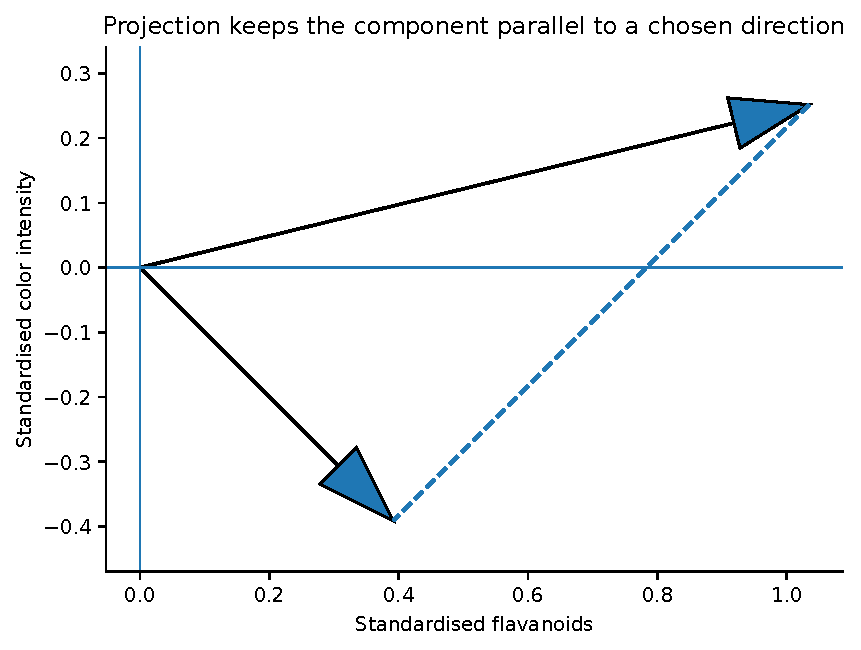
\includegraphics[width=0.60\linewidth]{figures_generated/math_vector_projection.pdf}
\end{utpfig}

\section{Means and variances summarise a distribution}
For observations $x_1,\ldots,x_n$, the sample mean is
\[
\bar{x}=\frac{1}{n}\sum_{i=1}^{n}x_i,
\]
and the sample variance is
\[
s^2=\frac{1}{n-1}\sum_{i=1}^{n}(x_i-\bar{x})^2.
\]
The mean is a balance point; variance measures average squared deviation around it. Squaring gives large deviations more weight and makes the quantity differentiable, which is useful in optimisation.

\section{Covariance links two variables}
Sample covariance is
\[
\operatorname{cov}(x,y)=\frac{1}{n-1}\sum_i(x_i-\bar{x})(y_i-\bar{y}).
\]
Positive covariance means above-average values of one variable tend to coincide with above-average values of the other. Correlation rescales covariance to a dimensionless number between $-1$ and $1$:
\[
r=\frac{\operatorname{cov}(x,y)}{s_xs_y}.
\]
Correlation measures linear association, not causation, and can miss important nonlinear patterns.

\section{Probability describes uncertainty over outcomes}
For an event $A$, probability satisfies $0\le P(A)\le1$. Conditional probability is
\[
P(A\mid B)=\frac{P(A\cap B)}{P(B)},
\]
provided $P(B)>0$. In classification, sensitivity, precision, and false-positive rates are all conditional probabilities with different conditioning events.

\begin{utpfig}[Conditioning changes the denominator]{Many classification metrics differ only in which subset becomes the denominator. Writing that subset explicitly prevents metric confusion.}{fig:math-conditioning}
\begin{tikzpicture}[x=\linewidth,y=1cm,
  stage/.style={draw=UTPBlue!70,fill=UTPPaleBlue,rounded corners=1.5mm,
    line width=0.6pt,text width=0.26\linewidth,minimum height=1.55cm,
    inner xsep=2.5mm,inner ysep=2mm,align=center,
    font=\scriptsize\color{UTPNavy}},
  connector/.style={line width=0.8pt,draw=UTPTeal,rounded corners=1.5mm},
  flow/.style={connector,-{Stealth[length=2mm,width=1.5mm]}}]
\node[stage] (all) at (0,0) {\textbf{All cases}\\[4pt]
  Choose the subset\\to condition on};
\node[stage] (actual) at (0.335,1.05) {\textbf{Actual positives}\\[4pt]
  Denominator: $TP+FN$};
\node[stage] (pred) at (0.335,-1.05) {\textbf{Predicted positives}\\[4pt]
  Denominator: $TP+FP$};
\node[stage,draw=UTPTeal!80,fill=UTPPaleTeal] (sens) at (0.670,1.05)
  {\textbf{Sensitivity}\\[4pt]
   $\displaystyle\frac{TP}{TP+FN}$};
\node[stage,draw=UTPOrange!80,fill=UTPPaleOrange] (prec) at (0.670,-1.05)
  {\textbf{Precision}\\[4pt]
   $\displaystyle\frac{TP}{TP+FP}$};
\coordinate (split) at (0.1675,0);
\draw[connector] (all.east) -- (split);
\draw[flow] (split) |- (actual.west);
\draw[flow] (split) |- (pred.west);
\draw[flow] (actual.east) -- (sens.west);
\draw[flow] (pred.east) -- (prec.west);
\end{tikzpicture}
\end{utpfig}

\section{Bayes' rule connects evidence and base rates}
Bayes' rule is
\[
P(A\mid B)=\frac{P(B\mid A)P(A)}{P(B)}.
\]
The term $P(A)$ is a base rate or prior probability. This is why a classifier with a low false-positive rate can still have modest precision when the positive class is rare: false positives are drawn from a much larger negative population.

\begin{workedexample}
Suppose a condition occurs in 1\% of cases. A test detects 95\% of true cases and has a 5\% false-positive rate. Out of 10,000 cases, roughly 95 true positives are expected, but about 495 false positives are also expected. Precision is therefore about $95/(95+495)\approx16\%$, despite high sensitivity.
\end{workedexample}

\section{Random variables have distributions}
A random variable associates possible outcomes with probabilities. A distribution describes which values are common, rare, or impossible. Expected value is a probability-weighted average; variance measures dispersion around that expectation.

Common models include Bernoulli for a binary outcome, Binomial for counts of successes under repeated trials, Normal for many continuous approximations, and Poisson for some event counts. Real data need not follow these models exactly for the concepts to be useful.

\section{Sampling distributions describe statistics, not raw observations}
A statistic such as $\bar{x}$ changes from sample to sample. Its distribution across hypothetical repeated samples is the \term{sampling distribution}. Standard errors and confidence intervals describe this statistic-to-statistic variation.

\begin{utpfig}[Sample means concentrate with larger samples]{The underlying population in this simulation is strongly skewed, yet averages from larger samples are more concentrated and increasingly symmetric.}{fig:math-clt}
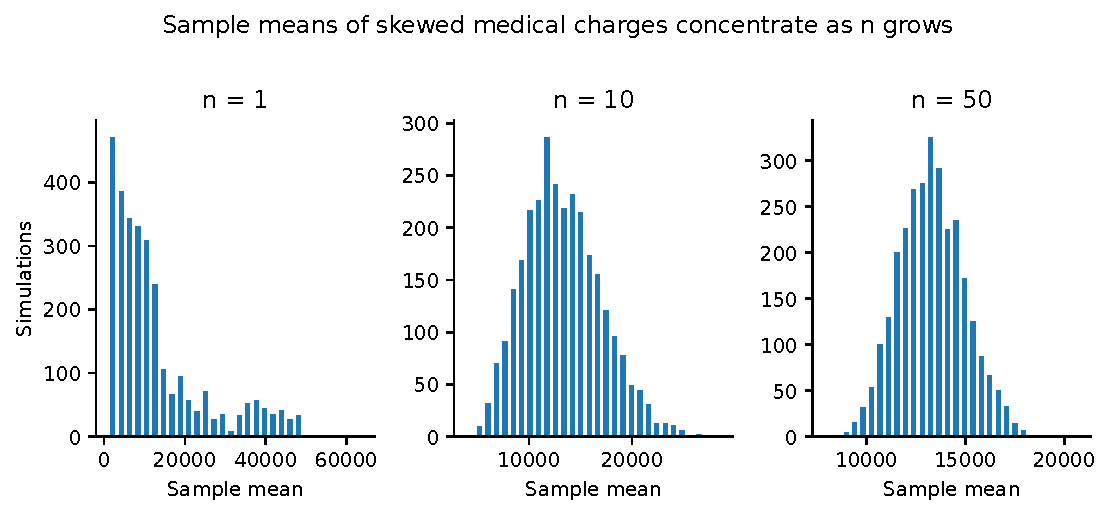
\includegraphics[width=0.82\linewidth]{figures_generated/math_clt.pdf}
\end{utpfig}

This is one reason averages can be estimated more precisely with larger samples. It does not mean the raw data become normal, and it does not correct systematic bias.

\section{Loss functions turn modelling into optimisation}
A model has parameters $\theta$. A \term{loss function} $L(\theta)$ measures how poorly the model fits the training objective. Training searches for parameter values with low loss.

For ordinary least squares,
\[
L(\beta_0,\beta_1)=\sum_i\left[y_i-(\beta_0+\beta_1x_i)\right]^2.
\]
For logistic regression, maximum likelihood is commonly expressed through the equivalent log-loss objective.

\begin{utpfig}[Optimisation searches for lower loss]{Each arrow represents a parameter update toward a lower region of the objective. Real models have many parameters, so the loss surface is high-dimensional.}{fig:math-optimisation}
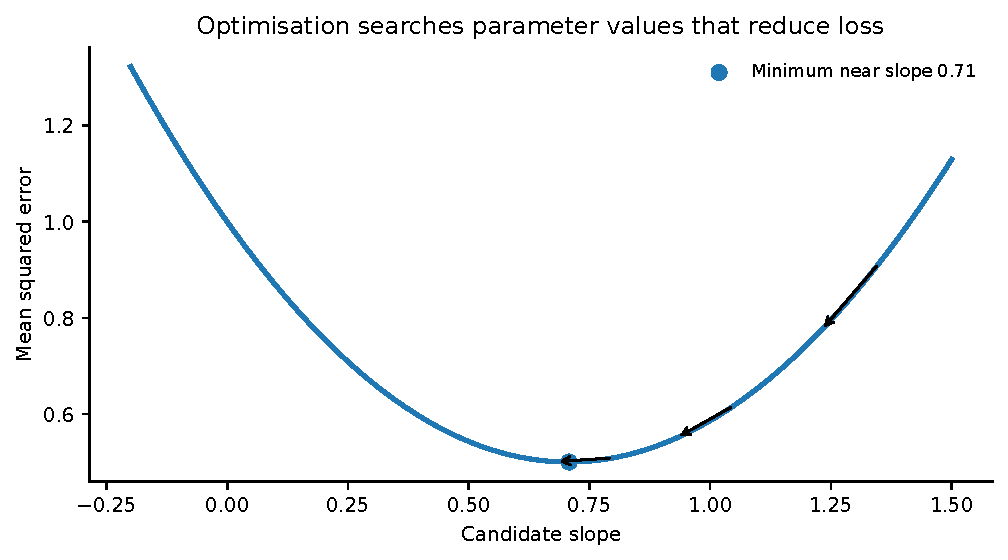
\includegraphics[width=0.78\linewidth]{figures_generated/math_loss_optimisation.pdf}
\end{utpfig}

\section{A derivative is a local rate of change}
For a one-dimensional function $f(\theta)$, the derivative $f'(\theta)$ tells how rapidly the function changes near $\theta$. In many dimensions, the gradient collects partial derivatives. Gradient-based optimisation moves parameters in a direction that reduces the objective.

The important data-science intuition is not symbolic differentiation by hand; it is that optimisation follows local information and can depend on scaling, learning rate, starting values, and the shape of the objective.

\section{Linear models combine features additively}
Multiple linear regression can be written
\[
\hat{\mathbf y}=X\boldsymbol{\beta}.
\]
Each coefficient changes the prediction associated with one feature while the others are held fixed. Interaction terms deliberately relax simple additivity by allowing the effect of one feature to depend on another.

\section{Logistic regression maps a linear score to a probability}
A linear score can take any real value. The logistic function maps that score to $(0,1)$:
\[
P(Y=1\mid X)=\frac{1}{1+e^{-\eta}},\qquad \eta=\beta_0+\beta_1x_1+\cdots+\beta_px_p.
\]
A threshold then converts the probability to an action or class label. Changing the threshold changes the balance between true-positive and false-positive rates.

\begin{utpfig}[One score model supports many thresholds]{The curve shows the family of true-positive and false-positive rates obtained by moving the decision threshold. There is no universally optimal point without an error-cost context.}{fig:math-threshold-tradeoff}
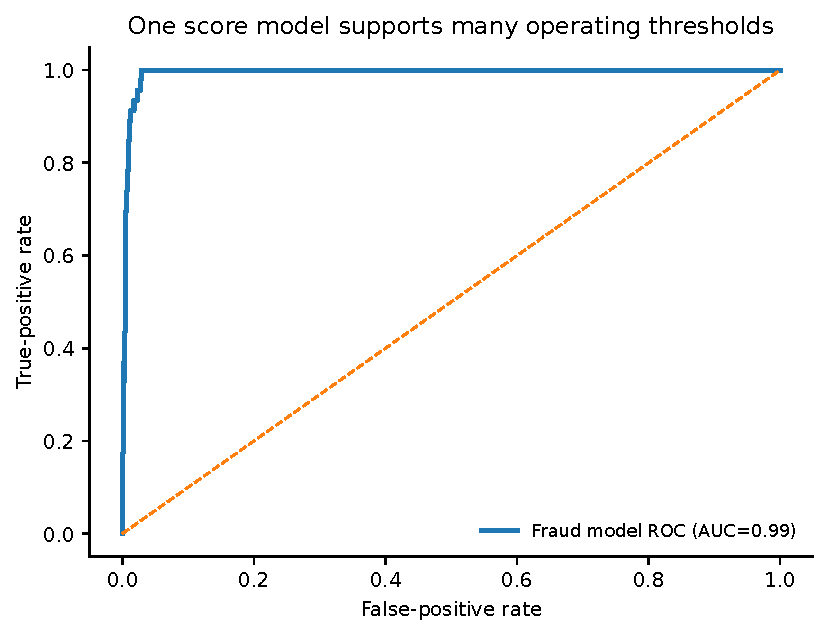
\includegraphics[width=0.62\linewidth]{figures_generated/math_threshold_tradeoff.pdf}
\end{utpfig}

\section{Eigenvectors explain the geometry of PCA}
The covariance matrix summarises how features vary together. PCA finds orthogonal directions---eigenvectors of the covariance or correlation matrix---ordered by the amount of variance associated with them. The corresponding eigenvalues quantify explained variance.

For practical interpretation:
\begin{itemize}
  \item scores are coordinates of observations in the component space;
  \item loadings describe how original features contribute to each component;
  \item explained-variance ratios quantify how much variation each component retains;
  \item scaling determines whether PCA emphasises absolute variance or variance in standardised units.
\end{itemize}

\section{Regularisation adds a preference to the objective}
Some models minimise a combination of prediction loss and a penalty on parameter magnitude. Ridge-style penalties use squared coefficients; lasso-style penalties use absolute coefficients. Regularisation can reduce variance and control complexity, especially when features are numerous or correlated.

Conceptually,
\[
\text{objective}=\text{prediction loss}+\lambda\times\text{complexity penalty}.
\]
The tuning parameter $\lambda$ controls the strength of the preference and should be selected using training-only validation procedures.

\section{The mathematical checklist}
When a formula appears in a data-science workflow, ask four questions:
\begin{enumerate}
  \item What objects does it take as input?
  \item What quantity does it produce?
  \item Which assumptions or coordinate choices affect it?
  \item How does that quantity change an analytical decision?
\end{enumerate}
This habit keeps mathematics connected to meaning rather than becoming isolated symbol manipulation.

\begin{chapterrecap}
\begin{itemize}
  \item Matrix notation is a compact description of rows, columns, features, and targets.
  \item Scaling changes geometry; dot products and projections connect directly to regression and PCA.
  \item Probability and conditional probability underpin inference and classification metrics.
  \item Sampling distributions explain why estimates vary; larger samples reduce random variability but not systematic bias.
  \item Model fitting is an optimisation problem in which loss functions and regularisation express what the algorithm is trying to minimise.
\end{itemize}
\end{chapterrecap}
